\documentclass[a4paper, 12pt]{article}
% Citações e Referências Bibliográficas 
\usepackage{apacite} 
\bibliographystyle{apacite} 
\usepackage{etoolbox} 
\renewcommand{\refname}{Referências Bibliográficas}

% Alfabeto e fonte 
\usepackage[utf8]{inputenc} 
\usepackage[T1]{fontenc} 
\usepackage{sectsty} 
\sectionfont{\fontsize{15}{15}\selectfont} % diminuir tamanho do nome das seções pra caber em duas colunas
\usepackage[brazilian]{babel} % Adiciona a opção "brazilian" para usar o idioma português brasileiro 
\addto\captionsbrazilian{% Redefine o título da seção de referências}
\renewcommand{\refname}{Referências Bibliográficas}% 
\renewcommand{\figurename}{\textbf{Figura}} 
\renewcommand{\tablename}{\textbf{Tabela}} 
\usepackage[format=hang,font=small,labelfont=bf]{caption}

% Formatação e margem 
\usepackage[top=3.0cm,bottom=2.0cm,left=2.0cm,right=2.0cm, headheight=1.5cm]{geometry} 
\usepackage{multicol}

% Coisas da matemática 
\usepackage{amsmath, amsfonts, amsthm, amssymb, physics}

% Desenhos, gráficos e tabelas 
\usepackage{tikz, siunitx, pbox, pgfplots, array, floatrow} 
\usetikzlibrary{quotes, angles} 
\floatsetup[table]{capposition=top} 
\usepackage[export]{adjustbox}

% Colocar equação dentro do retângulo 
\usepackage[most]{tcolorbox} 
\usepackage{framed}

\usepackage{fancyhdr} % Cabeçalhos e rodapés 
\usepackage{enumitem} % Enumeração 
\usepackage{graphicx} % Imagens 
\usepackage{titlesec} 
\usepackage{lipsum} % Para gerar texto de exemplo, você pode remover isso no documento final 
\usepackage{indentfirst} % Identar primeiro parágrafo 
\usepackage{float} % Formatação de Tabelas e Figuras 
\usepackage{relsize}
\usepackage{subcaption} % Para subfiguras

\pagestyle{fancy} 
\renewcommand{\footrulewidth}{.3pt} 
\renewcommand{\headrulewidth}{.3pt} 
\lhead{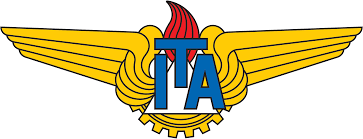
\includegraphics[height=1.2cm]{images/ITA.png}\vspace*{0.1cm}} 
\chead{\large CMC-12 Lab-5 \vspace*{0.1cm}} 
\rhead{} 
\cfoot{\thepage}

% Início do documento 
\begin{document} 
\thispagestyle{empty} 
\vspace*{2.15cm}

% Logo ITA
\begin{figure}[htb]
    \centering
    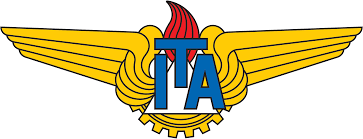
\includegraphics[scale=0.52]{images/ITA.png}
    
    \large Instituto Tecnológico de Aeronáutica
\end{figure}

\begin{center}
    \huge{CMC-12 – Exame Final} 
    
    \vspace{.5cm}
    \large Prof. Marcos Ricardo Omena de Albuquerque Maximo
    
    \vspace{1cm}
    \Huge Controlador Não Linear de Barra Articulada
    
    \vspace{.5cm}
    \Large Julho de 2025
    
    \vspace{.15cm}
    \large
    Danilo Miranda Oliveira \\
    Geison Vasconcelos Lira Filho \\
    José Alberto Feijão Tizon \\
\end{center}

\newpage
\setcounter{page}{1}


\section{Introdução}

Este relatório apresenta o projeto final desenvolvido na disciplina CMC-12, cujo objetivo é implementar e analisar um controlador não linear para o sistema que consiste em uma barra articulada sobre a qual uma argola pode deslizar livremente, sem atrito. O controle atua sobre o torque aplicado à barra, visando posicionar a argola em uma posição desejada \( x_r \) ao longo da barra, utilizando como única força externa a gravidade.

A solução implementada para projetar o controlador desse sistema permite que o projetista determine o tipo de controlador -- entre P, PI, PD, DI e PID -- e os requisitos de tempo de subida e de sobressinal para posicionar a argola numa barra infinita. Desse modo, é possível determinar o controlador mais eficaz para a barra do tamanho que se deseja projetar e verificar se os requisitos podem ser obedecidos para todas as posições da barra que se deseja projetar.



\section{Descrição do Sistema}

\subsection{Modelagem Física}

O sistema físico analisado consiste em uma barra rígida, com momento de inércia \( J \), articulada na posição \( x = 0 \) e assumida como infinitamente longa. Solidária a essa barra, uma argola de massa \( m \) desliza livremente, sem atrito. O controle do sistema é realizado por meio da aplicação de um torque \( \tau(t) \) na base da barra, o qual altera seu ângulo \( \theta(t) \) em relação à vertical. A única força externa considerada na modelagem é a força gravitacional atuando sobre a argola.

\subsection{Equações Dinâmicas Não Lineares}

No referencial solidário à barra, as forças atuantes sobre a argola ao longo do eixo \( x \) são a componente da força gravitacional, expressa como \( -mg \sin(\theta) \), e a força centrífuga decorrente da rotação da barra, dada por \( m \dot{\theta}^2 x \). Como se desprezam os atritos e forças perpendiculares à barra, como as forças de Coriolis e de Euler, que não influenciam a movimentação ao longo do eixo \( x \), a equação de movimento da argola no referencial rotativo é representada por:

\begin{equation}
    m \ddot{x} = -mg \sin(\theta) + m \dot{\theta}^2 x
\end{equation}

A dinâmica de rotação da barra é modelada por:

\begin{equation}
    \tau(t) = J \ddot{\theta}
\end{equation}

\subsection{Linearização via Espaço de Estados}

Para fins de análise e projeto de controladores lineares, é conveniente representar a dinâmica do sistema em espaço de estados. A partir do modelo não linear previamente obtido, consideram-se as seguintes equações que descrevem a dinâmica da argola e da barra:

\begin{align}
    m \ddot{x} &= -mg \sin(\theta) + m \dot{\theta}^2 x \label{eq:ddotx_nl} \\
    J \ddot{\theta} &= \tau \label{eq:ddottheta}
\end{align}

Definimos o vetor de estados como \( \mathbf{x} = [x \quad \dot{x} \quad \theta \quad \dot{\theta}]^\top \), a entrada como \( u = \tau \), e consideramos como saída a posição da argola \( y = x \).

A equação \eqref{eq:ddotx_nl}, dividida por \( m \), fornece:

\begin{equation}
    \ddot{x} = -g \sin(\theta) + \dot{\theta}^2 x
\end{equation}

De forma semelhante, da equação \eqref{eq:ddottheta}, temos:

\begin{equation}
    \ddot{\theta} = \frac{1}{J} \tau
\end{equation}

Substituindo as variáveis de estado, o sistema dinâmico pode ser reescrito como:

\begin{align}
    \dot{x}_1 &= x_2 \\
    \dot{x}_2 &= -g \sin(x_3) + x_4^2 x_1 \\
    \dot{x}_3 &= x_4 \\
    \dot{x}_4 &= \frac{1}{J} u
\end{align}

Com isso, obtém-se o modelo de espaço de estados não linear na forma compacta:

\begin{equation}
    \dot{\mathbf{x}} = f(\mathbf{x}, u), \quad y = h(\mathbf{x})
\end{equation}

Para linearizar o sistema, realiza-se uma expansão em série de Taylor de primeira ordem das funções \( f(\mathbf{x}, u) \) e \( h(\mathbf{x}) \) em torno do ponto de equilíbrio \( \mathbf{x}_e = \mathbf{0} \), \( u_e = 0 \). As matrizes do modelo linearizado são dadas por:

\begin{align}
    A &= \left.\frac{\partial f}{\partial \mathbf{x}}\right|_{\mathbf{x}_e, u_e} \qquad 
    B = \left.\frac{\partial f}{\partial u}\right|_{\mathbf{x}_e, u_e} \\
    C &= \left.\frac{\partial h}{\partial \mathbf{x}}\right|_{\mathbf{x}_e} \qquad\quad
    D = \left.\frac{\partial h}{\partial u}\right|_{u_e}
\end{align}

Calculando essas derivadas parciais, obtêm-se as seguintes matrizes:

\[
A = \begin{bmatrix}
0 & 1 & 0 & 0 \\
0 & 0 & -g & 0 \\
0 & 0 & 0 & 1 \\
0 & 0 & 0 & 0
\end{bmatrix}, \quad
B = \begin{bmatrix}
0 \\
0 \\
0 \\
\frac{1}{J}
\end{bmatrix}, \quad
C = \begin{bmatrix}
1 & 0 & 0 & 0
\end{bmatrix}, \quad
D = [0]
\]

Esse modelo linearizado descreve a dinâmica do sistema nas proximidades do ponto de equilíbrio. Ele será utilizado para o projeto dos controladores lineares na malha externa, uma vez que fornece uma aproximação acurada do comportamento local do sistema não linear original. A partir da modelagem em espaço de estados e da posterior aplicação de uma expansão em série de Taylor de primeira ordem em torno do ponto de equilíbrio \((\theta, \dot{\theta}, x, \dot{x}) = (0, 0, 0, 0)\), obtêm-se as equações linearizadas que descrevem a dinâmica local do sistema. Considerando pequenas oscilações e desprezando termos não lineares de ordem superior, a dinâmica reduz-se às seguintes equações diferenciais lineares:

\begin{equation}
    \ddot{x} = -g \cdot \theta
\end{equation}
\begin{equation}
    \ddot{\theta} = \frac{1}{J} \cdot \tau
\end{equation}

Essas expressões representam, respectivamente, a aceleração da argola em função da inclinação da barra e a aceleração angular da barra em função do torque aplicado. Tal forma linearizada é essencial para a síntese de controladores clássicos baseados em modelos lineares, como controladores PID ou estratégias de realimentação de estados.



\section{Projeto do Controlador}

\subsection{Estrutura em Malha Interna e Externa}
Devido à natureza hierárquica do sistema, em que a posição \( x \) depende do ângulo \( \theta \), que por sua vez depende do torque \( \tau \), adota-se uma abordagem com duas malhas de controle. A malha interna, mais rápida, é responsável por controlar o ângulo da barra a partir do torque aplicado. Para isso, utiliza-se um controlador proporcional com compensação de velocidade (P+V). Já a malha externa, mais lenta, controla a posição da argola ao longo da barra. São testados diferentes controladores (P, PI, PD, PID, Lead), todos com pré-filtro na referência.

\subsection{Controladores Utilizados nas Malhas}

A arquitetura de controle adotada é composta por uma estrutura hierárquica com duas malhas principais. A malha externa é responsável pelo controle da posição da argola e utiliza um controlador PID clássico, atuando sobre o erro de posição para gerar uma referência angular. Já a malha interna é dedicada ao controle da orientação da barra e implementa uma estratégia do tipo P+V. Essa estratégia consiste em duas realimentações aninhadas: uma proporcional sobre o ângulo da barra e outra proporcional sobre sua velocidade angular, funcionando respectivamente como ações de posição e velocidade.

Para o cálculo dos ganhos dos controladores, considera-se o modelo linearizado do sistema, no qual as não linearidades e forças centrífugas são desprezadas. Os parâmetros são calculados de forma analítica, a partir dos requisitos de desempenho definidos para o sistema. Posteriormente, o projeto é validado no ambiente Simulink, onde o modelo exato do sistema é simulado, incluindo as não linearidades e a força centrífuga que foram omitidas na linearização. Dessa forma, verifica-se se o controlador projetado atende adequadamente ao desempenho esperado quando aplicado ao sistema real.


\section{Simulações e Resultados}

\subsection{Descrição dos Casos Simulados}
Foram simulados diferentes casos, variando-se as condições iniciais da argola e da barra, bem como os valores de referência \( x_r \). O objetivo foi verificar o comportamento do sistema sob diferentes regimes de operação e testar a robustez dos controladores projetados.

\subsection{Resultados}
Os gráficos obtidos mostram a evolução temporal da posição da argola \( x(t) \), do ângulo da barra \( \theta(t) \), do torque aplicado \( \tau(t) \), bem como do erro de rastreamento \( x(t) - x_r \). Esses resultados permitem avaliar o desempenho do sistema de controle em termos de estabilidade, precisão e tempo de resposta.

\subsection{Análise dos Resultados}
A partir das simulações, observa-se o comportamento dinâmico do sistema frente a diferentes controladores e referências. São analisados aspectos como a estabilidade do sistema, o tempo de acomodação, a presença de oscilações, e a robustez frente a variações nos parâmetros do modelo. Resultados satisfatórios indicam que a estratégia de controle adotada foi eficaz dentro das condições simuladas.

\section{Conclusão}
O desenvolvimento deste projeto permitiu compreender os principais desafios envolvidos no controle de sistemas não lineares, especialmente na presença de malhas hierárquicas e interdependentes. A estratégia de controle adotada, com malhas interna e externa, mostrou-se efetiva para garantir o rastreamento da posição desejada pela argola, mesmo em condições adversas. Como possíveis extensões do trabalho, sugere-se a análise do sistema com perturbações externas, como atrito ou impa


\end{document}
